\documentclass{article}

\usepackage{indentfirst}
\usepackage{color}
\usepackage{graphicx}
\usepackage{amsmath}
\usepackage{epsfig}
\usepackage{geometry}
\usepackage{setspace}
\usepackage{xcolor}
\usepackage{listings}

\lstset{%
alsolanguage=Python,
% language={[Visual]Python},       %language为,还有{[Visual]Python}
%alsolanguage=[ANSI]C,      %可以添加很多个alsolanguage,如alsolanguage=matlab,alsolanguage=VHDL等
%alsolanguage= tcl,
alsolanguage= XML,
tabsize=4, %
  frame=shadowbox, %把代码用带有阴影的框圈起来
  commentstyle=\color{red!50!green!50!blue!50},%浅灰色的注释
  rulesepcolor=\color{red!20!green!20!blue!20},%代码块边框为淡青色
  keywordstyle=\color{blue!90}\bfseries, %代码关键字的颜色为蓝色,粗体
  showstringspaces=false,%不显示代码字符串中间的空格标记
  stringstyle=\ttfamily, % 代码字符串的特殊格式
  keepspaces=true, %
  breakindent=22pt, %
  numbers=left,%左侧显示行号 往左靠,还可以为right,或none,即不加行号
  stepnumber=1,%若设置为2,则显示行号为1,3,5,即stepnumber为公差,默认stepnumber=1
  %numberstyle=\tiny, %行号字体用小号
  numberstyle={\color[RGB]{0,192,192}\tiny} ,%设置行号的大小,大小有tiny,scriptsize,footnotesize,small,normalsize,large等
  numbersep=8pt,  %设置行号与代码的距离,默认是5pt
  basicstyle=\footnotesize, % 这句设置代码的大小
  showspaces=false, %
  flexiblecolumns=true, %
  breaklines=true, %对过长的代码自动换行
  breakautoindent=true,%
  breakindent=4em, %
  escapebegin=\begin{CJK*}{GBK}{hei},escapeend=\end{CJK*},
  aboveskip=1em, %代码块边框
  tabsize=2,
  showstringspaces=false, %不显示字符串中的空格
  backgroundcolor=\color[RGB]{245,245,244},   %代码背景色
  %backgroundcolor=\color[rgb]{0.91,0.91,0.91}    %添加背景色
  escapeinside=``,  %在``里显示中文
  %% added by http://bbs.ctex.org/viewthread.php?tid=53451
  fontadjust,
  captionpos=t,
  framextopmargin=2pt,framexbottommargin=2pt,abovecaptionskip=-3pt,belowcaptionskip=3pt,
  xleftmargin=4em,xrightmargin=4em, % 设定listing左右的空白
  texcl=true,
  % 设定中文冲突,断行,列模式,数学环境输入,listing数字的样式
  extendedchars=false,columns=flexible,mathescape=true
  % numbersep=-1em
}

\geometry{left=2cm,right=2cm,top=2cm,bottom=2cm}
\begin{document}
\begin{spacing}{1.2}
\vspace*{0.25cm}

\thispagestyle{empty}

\begin{center}
\hrulefill

\thispagestyle{empty}


\begin{large}
\sc{CompSci 261P \\ Data Structures}
\end{large}

\hrulefill

\vspace*{5cm}
\begin{Large}
\sc{{Data Retrieval Efficiency Comparison}}

\sc{{among}}

\sc{{Binary Search Tree, AVL Tree and B- Tree}}
\end{Large}

\vspace{2em}

\end{center}


\vfill

\begin{table}[h!]
\flushleft
\begin{tabular}{lll}
Name: Xingyou Ji \hspace*{2em}
\\
Date: 9 November 2019

\end{tabular}
\end{table}

\hfill

\newpage
\section{Summary}
This project will focus on the efficiency to retrieve records from binary search tree, AVL tree and B- tree. Specifically, I will implement binary search tree, AVL tree and B- tree, and perform data retrieval tests for all these tree trees to validate B- tree has the best performance.
\section{Underlying Problem}
Binary tree is a common and fundamental data structure to store data, and it supports $O(\log n)$ data retrieval in average case. However, if the binary search tree is unbalanced as shown in Fig \ref{unbalanced}, the worst case running time of data retrieval can go up to $O(n)$. Therefore, if the data size is sufficiently large, users cannot afford the worst case running time.
\begin{figure}[!h]
    \centering
    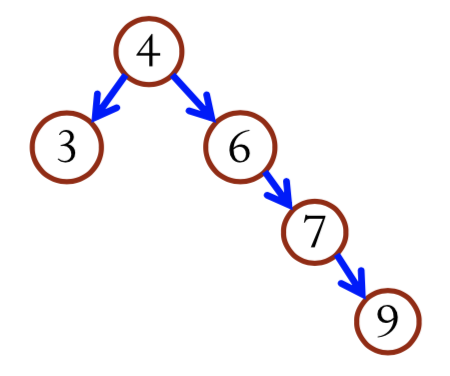
\includegraphics[width=0.2\textwidth]{unbalanced.png}
    \caption{Unblanced binary search tree}
    \label{unbalanced}
\end{figure}

AVL tree is designed to fix the above issue by enforcing the maximum difference between left and right subtrees to be no more than 1. 

Modern databases, such as SQL, use B- tree to store data. The advantage of a B- tree is to reduce the number of nodes, so that fewer I/O processes are performed. 

In this project, I will implement binary search tree, AVL tree as well as B- tree, and test their efficiency on data retrieval to see whether B- tree has the best performance.

\section{Evaluation Method}
I propose to use a counter to record how many nodes are visited when doing a retrieval operation. The reason why I choose to record the number of visited nodes rather than operation time is that the runnimg time depends on the complexity of the data structure. So, as the B- tree has a more complex structure, it could happen that it takes longer time to do the opertion. However, in real-life appications, the most time-consuming step is I/O, which is equivalent to the number of visited nodes in this project. Therefore, in order to validate that B- tree is indeed the best option for databases to use, it is wise to compare the number of visited nodes.

\section{Proposed Test}
I propose to generate $8$ files, each containing $10, 50, 100, 500, 1000, 5000, 10000, 50000$ random data. Denote the file with size $n$ as $F_n$. I will first store these $n$ records into binary search tree, AVL tree and B- tree. Then, I will randomly generate an index $i$, and do a retrieval of record $F_n[i]$ for all three trees, and record the number of visited nodes in each tree.

In order to show the worst case of binary search tree, I will perform one additional test, that is, store 100 sorted elements in these three trees, and record their corresponding number of visited nodes.

\end{spacing}
\end{document}